\small\setchapterpreamble[u]{\margintoc}\normalsize
\chapter{Materials and software}
\labch{materials}
\label{sec:materials}

\section*{About this chapter}

This chapter comprises the specifications of sensors used throughout this research work, the drawbacks of each of them and how these were solved. The core data of this dissertation is imagery taken from \acrshort{uas}s; therefore, this section is dedicated to both imagers and drones applied to capturing input data. Materials either belong to the Graphics and Geomatics Group at the University of Jaén (TIC-144) or the Science and Technology Faculty at the University of Trás-os Montes e Alto Douro (Vila Real, Portugal). 

\begin{marginfigure}[.5cm]
    \centering
	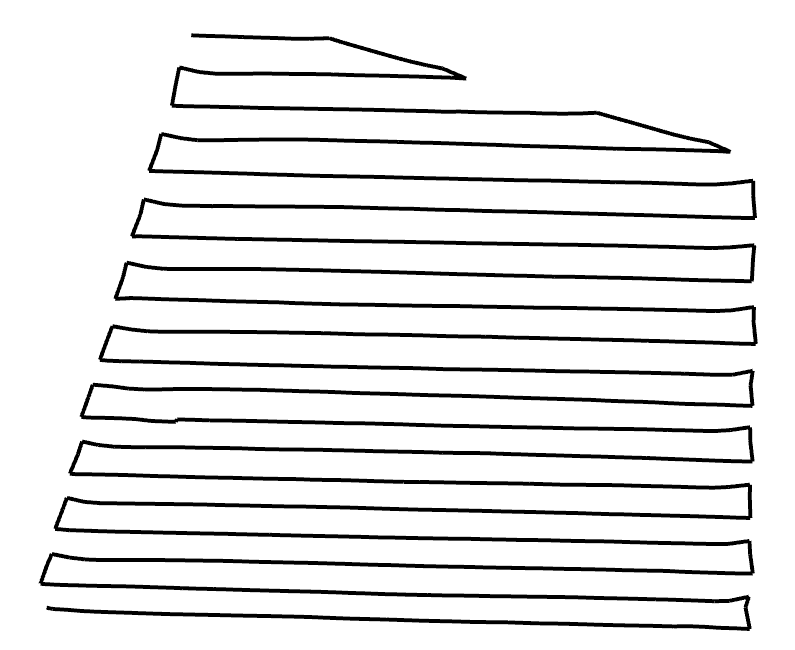
\includegraphics[width=.8\linewidth]{figs/materials/boustrophedon.png}
	\caption{Boustrophedon path planning.}
    \label{fig:boustrophedon}
\end{marginfigure}
\section{UAS platforms}

The \acrshort{uas} platforms used during any of the surveys are following described. The first belongs to the University of Jaén whereas the latter two have been used over the region of Vila Real, Portugal.

\subsection{DJI Matrice 210}

\begin{marginfigure}[0.1cm]
	\includegraphics[width=\linewidth]{figs/materials/dji_matrice_210.jpg}
	\caption{Quadcopter DJI Matrice 210 equipped with a thermal sensor, DJI Zenmuse XT2, and the Parrot Sequoia multispectral sensor.}
    \label{fig:dji_matrice_210}
\end{marginfigure}
DJI Matrice 210 is a quadcopter drone that has been coupled with multispectral and thermal imagers. Missions were planned and launched using DroneDeploy (California, CA, USA) in the remote control device. Flights have been typically established at 45-50 \si{\meter} from the take-off position, whereas the path planning has always been set to define a Boustrophedon path (see Figure \ref{fig:boustrophedon}), i.e., back and forth parallel lines. View direction was configured as \textit{nadir} when possible, with high frontal ($\sim$90\%) and side ($\sim$85\%) overlap to ensure images can be matched.

\subsection{DJI Matrice 600 Pro}

DJI Matrice 600 Pro (M600) is a hexacopter which has been used to record hyperspectral data with a Nano-Hyperspec device. It is equipped with a Ronin-MX gimbal to minimize geometric distortions in HSI acquisition. Its location was captured at different timestamps using two \acrshort{gps} in the arms, and its altitude was determined by the other three \acrshort{gps} mounted on the upper plate. Angular data (yaw, roll and pitch angles) were recorded using an \acrshort{imu}. With this equipment, the flight autonomy is approximately 20 \si{\minute} \cite{sousa_uav-based_2022}. Flights were planned using Universal Ground Control Station at an altitude of 50 \si{\meter} with a 40\% side overlap for the observation of vineyard rows and the University of Trás-os Montes e Alto Douro campus.
\begin{marginfigure}[-3.0cm]
	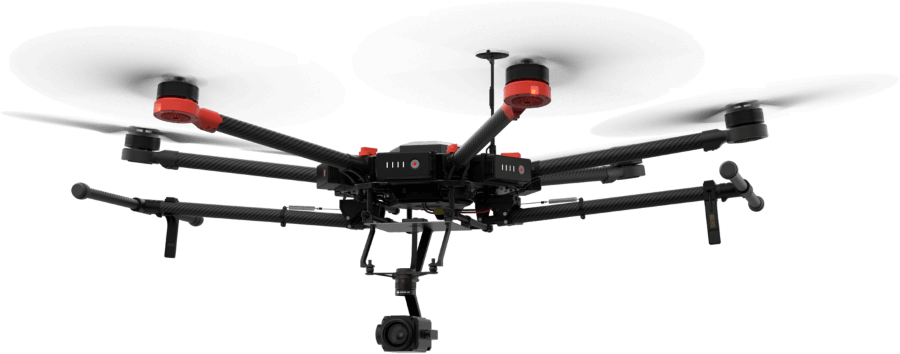
\includegraphics{figs/materials/dji_matrice_600_pro.png}
	\caption{Hexacopter DJI Matrice 600 Pro.}
	\label{fig:dji_matrice_600_pro}
\end{marginfigure}

\subsection{DJI Phantom 4}

\begin{marginfigure}[.1cm]
	\includegraphics{figs/materials/phantom.png}
	\caption{Quadcopter DJI Phantom 4.}
	\label{fig:dji_phantom4}
\end{marginfigure}
DJI Phantom 4 is a quadcopter with an integrated \acrshort{cmos} camera of 2.8 \si{\milli\meter} optical lens and 12.4 megapixels (MP). Images have a resolution of $4000 \times 3000$ px, whereas video recording is also allowed at different qualities, including Ultra High-Definition (\acrshort{uhd}: $4096 \times 2160$ px at 24/25 frames per second (\acrshort{fps})). It can fly up to an altitude of 6000 \si{\meter} above water level with an autonomy of approximately 28 \si{\minute}. Integration with other sensors such as the Parrot Sequoia is not trivial as it requires the design of a coupling platform and feeding the sensor with an energy source, e.g., a battery. Although it is possible to integrate further sensors, this \acrshort{uas} has only been applied to \acrshort{rgb} recording with the integrated camera. Path planning has been performed with DroneDeploy (DroneDeploy, San Francisco, CA, USA).

\section{Sensors}

\subsection{Parrot Sequoia}

\begin{marginfigure}[.2cm]
	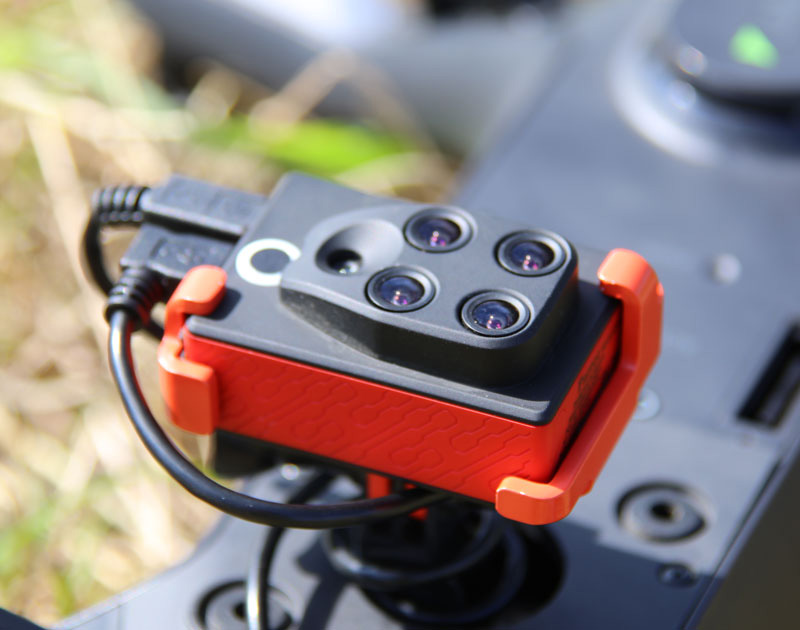
\includegraphics{figs/materials/sequoia_parrot.jpg}
	\caption{Parrot Sequoia multispectral device.}
	\label{fig:parrot_sequoia}
\end{marginfigure}
Parrot Sequoia is a multispectral sensor from Parrot that has been mainly advertised as an imager for Precision Agriculture. It covers four different spectral bands (see Table \ref{table:parrot_sequoia}) using wide-angle lenses with a focal length of $\sim$4 \si{\milli\meter}. Along with multispectral observations, it is also able to capture information in the visible range with an \acrshort{rgb} sensor of 15.9 MP and a focal length of 4.88 \si{\milli\meter}. The latter is captured in rolling shutter mode, and therefore, not all parts of the image are captured at the same time. Thus, the \acrshort{uas} pace ought to be configured low enough to avoid effects such as wobble, skew as well as spatial and temporal distortion. Regarding the dimensionality of outputs, the resolution is 1280$\times$960 px and 4608$\times$3456 px for multispectral and visible imagery, respectively. Examples of shots from the Parrot Sequoia device for two different study areas are depicted in Figure \ref{fig:multispectral_samples}. 

\begin{figure*}[ht]
	\includegraphics[width=\linewidth]{figs/materials/multispectral_samples.png}
	\caption{\acrshort{rgb} and multispectral bands as captured from a Parrot Sequoia device.}
	\label{fig:multispectral_samples}
\end{figure*}

\renewcommand{\arraystretch}{1.2}
\begin{table}[ht]
    \small
    \caption{Specifications of the Parrot Sequoia multispectral device.}
    \label{table:parrot_sequoia}
    \begin{tabular}{llll}
        \toprule
        Band & Spectral range & Image size & Focal length\\
        \midrule
        Green (GRE) & $530-570$ \si{\nano\meter} & \multirow{4}{*}{$1280 \times 960$ px} & \multirow{4}{*}{3.8 \si{\milli\meter}}\\
        Red (RED) & $640-680$ \si{\nano\meter} & & \\
        Red-edge (\acrshort{reg}) & $730-740$ \si{\nano\meter} & & \\
        Near-infrared (\acrshort{nir}) & $770-810$ \si{\nano\meter} & &\\
        \cmidrule{1-4}
        Visible (RGB) & Visible & $4608 \times 3456$ px & 4.88 \si{\milli\meter}\\
        \bottomrule
    \end{tabular}
\end{table}
\renewcommand{\arraystretch}{1}

Wide-angle lenses cover wider areas with a single shot, but also present visual distortions such as the well-known fisheye effect (Figure \ref{fig:fisheye_sample}). Surfaces with rectilinear features are depicted as domed with this distortion, especially for features close to the image corners. It can be corrected with a transformation matrix that creates an image of the same dimensionality, whose pixels carry out the interpolated colour from several pixels of the source image. Remark that interpolation algorithms are required since the transformation of $x' \in \mathbb{N}$ yields $x \in \mathbb{R}$.

\begin{figure}[ht]
	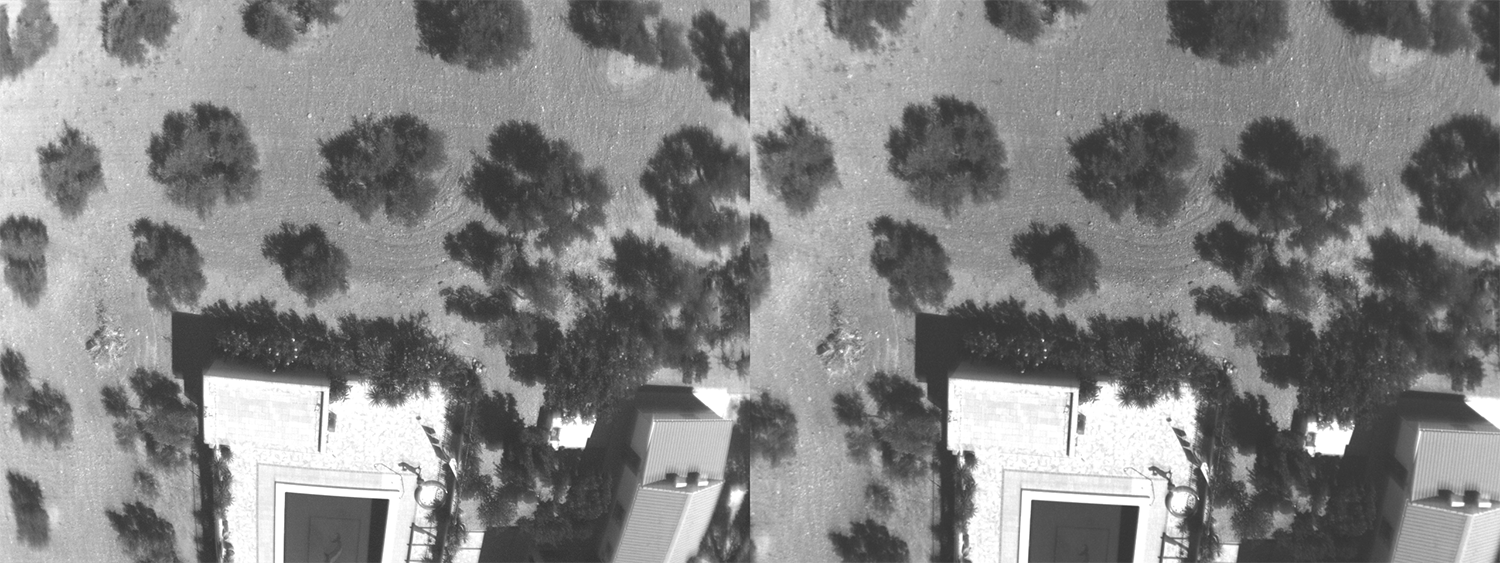
\includegraphics{figs/materials/fisheye_sample.png}
	\caption{Image with fisheye effect and the target image after the removal of such a distortion.}
	\label{fig:fisheye_sample}
\end{figure}

Figure \ref{fig:fisheye_model} shows this relation on the basis of $\alpha$ and $\beta$ angles. $\beta$ is the angle between the optical axis and the segment that goes from the lens' origin, $c_o$, to a source point, $p$, that is paired with a target point, $p'$. For the target image, $\alpha$ is used instead of $\beta$, and $p$ is transformed to $p'$. Note that $p \neq p'$, though both lie on the segment $\overline{c_p p}$. The explained transformation push points into $c_p$, and it is formally defined by means of $f(x) = x'$ and $f(y) = y'$. Therefore, $\alpha$ is easily calculated with trigonometry using the optical axis and any segment $\overline{c\textsubscript{o}p'}$, as shown in Equation \ref{eq:alpha}. Besides this, $\alpha$ is normalized in [0, 1]:
\begin{equation}
\begin{split}
\label{eq:alpha}
\alpha & = \frac{2}{\pi} * \tan^{-1}(\frac{\sqrt{(p'_x-{c_p}_x)^2 + (p'_y-{c_p}_y)^2}}{f}) = \frac{2}{\pi} * \tan^{-1}(\frac{r}{f})
\end{split}
\end{equation}

\begin{figure}[ht]
	\centering
	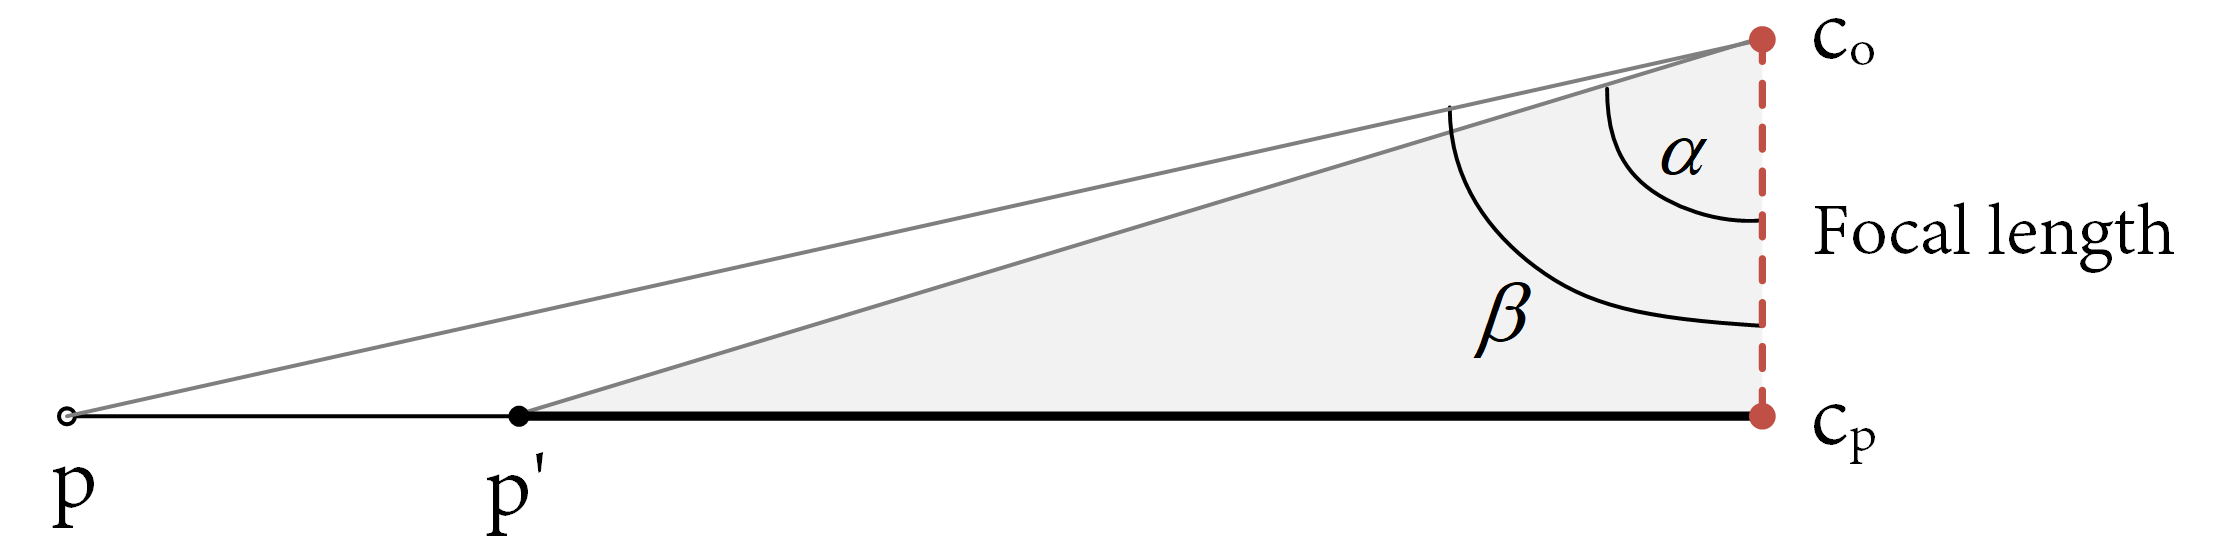
\includegraphics[width=\linewidth]{figs/materials/fisheye_model_2.png}
	\caption{Relation between a pixel from the target image, $p'$, and another from the source image, $p$.}
	\label{fig:fisheye_model}
\end{figure}

Then, four polynomial coefficients ($k_1, k_2, k_3, k_4$) are read from the image metadata to compute the angle $\beta$ between the optical axis and the segment $\overline{c\textsubscript{o}p}$, as expressed in Equation \ref{eq:beta}. Note that this correction model is provided by Parrot.
\begin{equation}
\label{eq:beta}
\beta = k_1 + k_2 * \alpha + k_3 * \alpha ^ 2 + k_4 * \alpha ^ 3
\end{equation}

\begin{marginfigure}[-1.5cm]
	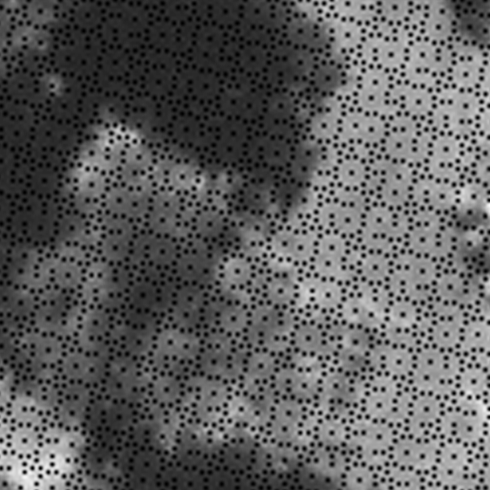
\includegraphics{figs/materials/inverse_mapping.png}
	\caption{Undetermined values are obtained when the undistortion process is carried out from the source image to the target one.}
	\label{fig:inverse_mapping}
\end{marginfigure}
The new image has the same size, with $p'$ receiving the colour of $p$. It is relevant to perform this operation in this order, $p' \gets p$, to determine the colour of each pixel. Instead, the inverse mapping ($p \rightarrow p'$) leaves undetermined values since multiple pixels from the source image could be mapped to the same pixel in the target image (see Figure \ref{fig:inverse_mapping}). Thus, the last step is to map every $(x', y')$ to $(x, y)$, with $x, y \in \mathbb{R}$. A bilinear interpolation algorithm is used to solve the problem of accessing float-point indices from an image.

\subsection{DJI Zenmuse XT2}

\begin{marginfigure}[.1cm]
	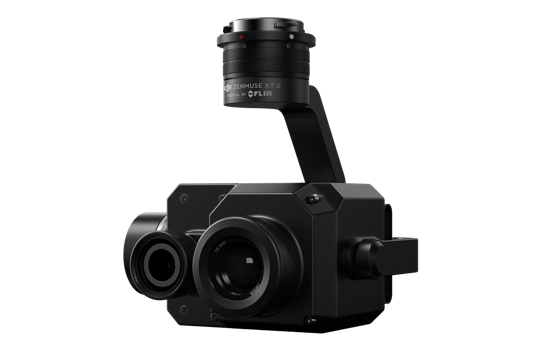
\includegraphics{figs/materials/zenmuse_xt2.png}
	\caption{DJI Zenmuse XT2 dual-payload sensor.}
	\label{fig:zenmuse_xt2}
\end{marginfigure}
DJI Zenmuse XT2 is a dual payload device that includes \acrshort{rgb} and thermal cameras. The \acrshort{rgb} camera provides high-resolution images (\acrshort{cmos} sensor with 12 MP) with a focal length of 8 \si{\milli\meter}, whereas the thermal imager acquires results of lower resolution (Table \ref{table:zenmuse_xt2}) in the \acrshort{lwir} interval from surfaces whose temperature range between $-40^\circ$ and $550^\circ$. \acrshort{ir} radiation was configured to be represented as grayscale values enhanced by edges from objects. The device as a whole is stabilized by a gimbal. Both types of images are acquired synchronously and despite this, there exist differences among them due to possible minor delays in the triggering, drone movement and distance of lenses. \acrshort{rgb} images are stored in Joint Photographic Experts Group (\acrshort{jpeg}) file format, whereas thermal imagery is either stored as \acrshort{rjpeg} (Radiometric JPEG) or \acrshort{tiff} (Tag Image File Format). The first allows calculating the temperature as a function of a large number of parameters, whereas the latter saves the temperature as observed and configured. Hence, the first is better if some of the parameters must be tweaked on post-processing, e.g., the atmospheric temperature. As occurred for previous devices, these images are also affected by distortions either from wide-angle or very narrow lenses.

\renewcommand{\arraystretch}{1.2}
\begin{table}[ht]
    \caption{Specifications of images acquired by a DJI Zenmuse XT2 device.}
    \label{table:zenmuse_xt2}
    \begin{tabular}{llll}
        \toprule
        Band & Spectral range & Image size & Focal length\\
        \midrule
        Thermal & $750-1,350$ \si{\nano\meter} & $640 \times 512$ px & 19 \si{\milli\meter}\\
        Visible (\acrshort{rgb}) & Visible & $4000 \times 3000$ px & 8 \si{\milli\meter}\\
        \bottomrule
    \end{tabular}
\end{table}
\renewcommand{\arraystretch}{1}

\subsubsection{Geometric correction}

Images captured by the DJI Zenmuse XT2 are affected by distortions that must be removed for later projection procedures. First, thermographic imagery presents pincushion distortion as a result of the narrow field of view ($32^\circ \times 26^\circ$), whereas \acrshort{rgb} images are distorted following the barrel effect. Unlike Parrot, the camera manufacturer does not define a specific distortion model and thus can be removed as for any other image. Geometric distortions can be removed by means of the camera matrix, $K$, as well as radial and tangential distortion coefficients, $(k_1, k_2, p_1, p_2, k_3)$. Also in contrast to Parrot Sequoia, these factors are not provided as image metadata. Instead, they must be determined through calibration and as such are estimated as part of the initial processing of \acrshort{sfm}. Whether an image follows a pincushion or barrel distortion model is determined by the main distortion coefficient, $k_1$. It is below zero for thermal images, i.e., surfaces are not rectilinear; instead, they bow inwards as a consequence of the pincushion distortion. On the other hand, \acrshort{rgb} images have a barrel effect that is removed in the same way, though their principal radial coefficient, $k_1$, is greater than zero. For the latter, surfaces are bowed outwards and therefore, removing the distortion does not require decimating the image (Figure \ref{fig:rgb_xt2_undistortion}).

\begin{figure}
    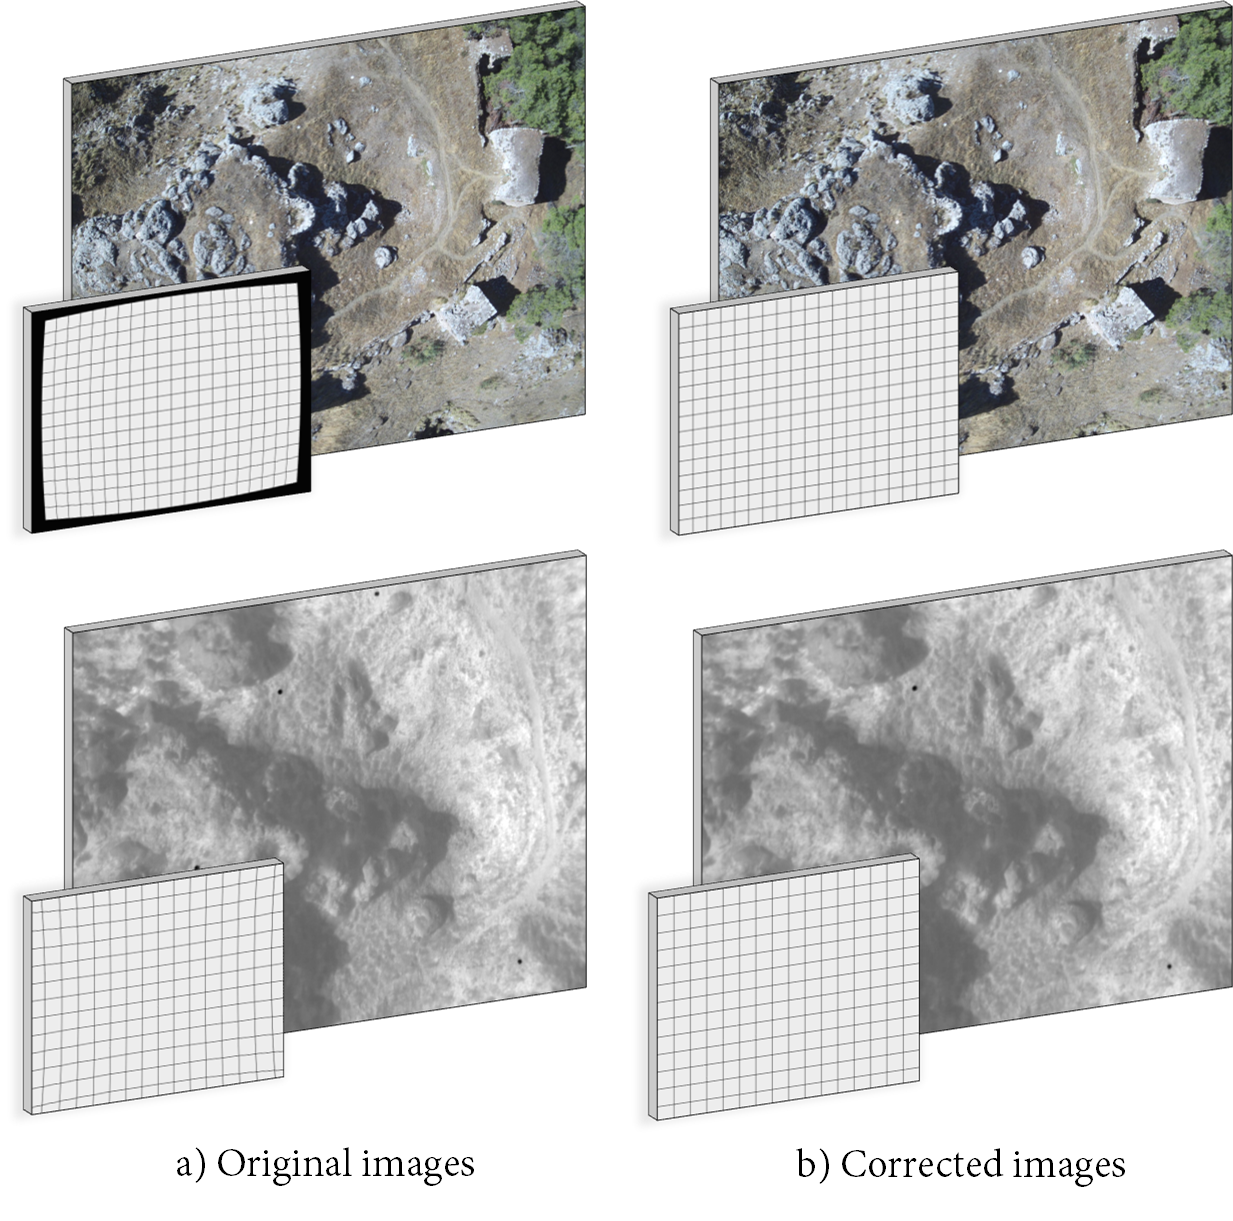
\includegraphics{figs/materials/thermal_distortion.png}
    \caption{Result of geometrical corrections regarding visible and thermal imagery. Barrel and pincushion effects are depicted through distorted grids.}
    \label{fig:thermal_rgb_distortion}
\end{figure}

\begin{figure}[ht]
	\centering
	\includegraphics{figs/materials/rgb_xt2_undistortion.png}
	\caption{Comparison of distorted \acrshort{rgb} image and the corrected result.}
	\label{fig:rgb_xt2_undistortion}
\end{figure}

As depicted in Figure \ref{fig:thermal_rgb_distortion}, corrected images have null values if the result has a lower dimensionality than the starting image. Hence, the minimum area that presents non-null colours can be determined by calculating the new corners of the image and subsequently cropping it (Equation \ref{eq:matrix_corners}). As a result, corrected images can have lower resolution than the initial ones, as occurs for thermal images. Figure \ref{fig:thermal_undistortion} compares three stages of the correction procedure. 
\begin{gather}
    \small
    \begin{aligned}
    \label{eq:matrix_corners}
    \min_x &= \max \{\max_x \{M \cdot [0, 0, 1]^\mathsf{T}, M \cdot [0, h - 1, 1]^\mathsf{T}\}, \min_x\}\\
    \min_y &= \max \{\max_y\{M \cdot [0, 0, 1]^\mathsf{T}, M \cdot [w - 1, 0, 1]^\mathsf{T}\}, \min_y\}\\
    \max_x &= \min \{\min_x\{M \cdot [w - 1, 0, 1]^\mathsf{T}, M \cdot [w - 1, h - 1, 1]^\mathsf{T}\}, \max_x\}\\
    \max_y &= \min \{\min_y\{M \cdot [0, h - 1, 1]^\mathsf{T}, M \cdot [w - 1, h - 1, 1]^\mathsf{T}\}, \max_y\}\\
    \end{aligned}
    \normalsize
\end{gather}

Distortion is removed by following the transformations defined in Equations \ref{eq:distortion_removal}, whereas the inverse produce can also be followed to guarantee every pixel is mapped to a colour.
\begin{gather}
    \label{eq:distortion_removal}
    \begin{aligned}
    \begin{bmatrix} 
        x'\\y'\\ z'
    \end{bmatrix}
    =& 
    \begin{bmatrix}
        \frac{x - c_x}{f_x}\\\frac{y - c_y}{f_y}\\ 1
    \end{bmatrix}
    = 
    \inv{K} \begin{bmatrix}
        x\\ y\\ 1
    \end{bmatrix}\\
    r^2 =& \hspace{1mm} {x'}^2 + {y'}^2\\
    x_u =& \hspace{1mm} x' \cdot (1 + k_1r^2 + k_2r^4 + k_3r^6) + 2p_1{x'}{y'} + p_2(r^2 + 2{x'}^2)\\
    y_u =& \hspace{1mm} y' \cdot (1 + k_1r^2 + k_2r^4 + k_3r^6) + p_1(r^2 + 2{y'}^2) +2p_2{x'}{y'}
    \end{aligned}
\end{gather}

\begin{figure}[hbt]
	\centering
	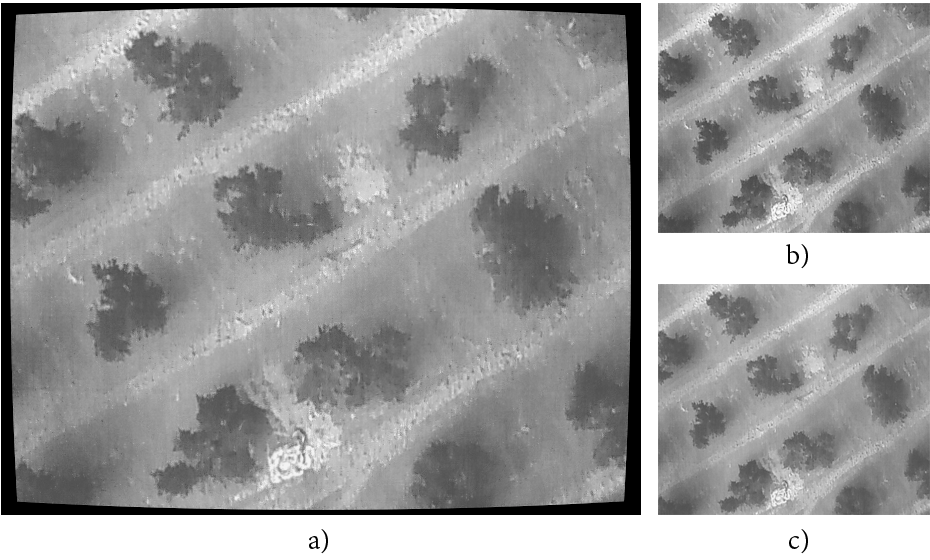
\includegraphics[width=\linewidth]{figs/materials/thermal_distortion_2.png}
	\caption{Comparison of a) free of distortion thermal image with blank values preserving the original size, b) distorted thermal image and c) free of distortion thermal image with reduced size.}
	\label{fig:thermal_undistortion}
\end{figure}

$x_u, y_u$ refer to coordinates from an image without distortion effects, although corrected images are generated in the opposite order. For each pixel, defined by its integer coordinates, the distorted pixel from where colour is obtained, $x_{d}, y_{d} \in{\mathbb{R}}$, is calculated using Equation \ref{eq:distortion_removal_2}. Again, an interpolation such as the bilinear function is required in this process.
\begin{gather}
    \label{eq:distortion_removal_2}
    \begin{aligned}
        \begin{bmatrix} 
            x_d, y_d, 1
        \end{bmatrix}^\intercal 
        =
        \begin{bmatrix}
            {x'}f_x + c_x, {y'}f_y + c_y, 1
        \end{bmatrix}^\intercal
        =
        \hspace{1mm} K \begin{bmatrix}
            {x'}, {y'}, 1
        \end{bmatrix}^\intercal
    \end{aligned}
\end{gather}

\subsubsection{Radiometric correction}

This section is mainly referred to thermography stored using the proprietary \acrshort{rjpeg} file format. With this encoding, images are depicted as a normalized representation of the temperature observed in the scene. However, these values are not the observed temperature. Still, the temperature can be extracted using the metadata of \acrshort{rjpeg} files. Thermal cameras record the radiation emitted from the objects' surface, either it comes from the object itself or surrounding objects. Additionally, it is conditioned by several environmental parameters, such as air humidity, air temperature and background temperature. Besides this, the object reflectivity and emissivity, as well as the distance between the surface and the camera are also relevant to the final measurements \cite{vollmer_infrared_2017}. Each manufacturer models the transmissivity of the atmosphere through a theoretical or empirical law, using some constant values embedded in the image metadata \cite{teza_evaluation_2019}. Consequently, several parameters must be retrieved from the embedded data, including the emissivity, atmospheric temperature, reflected apparent temperature, infrared window temperature, infrared window transmission, relative humidity, Planck's constants ($P_{R1}$, $P_{R2}$, $P_O$, $P_F$, $P_B$) and atmospheric transmission constants ($\alpha_0$, $\alpha_1$, $\beta_0$, $\beta_1$, $\mathcal{X}$). Most of them are calibrated by the manufacturer against a blackbody radiation source and thus only a few parameters can be adjusted. The final temperature $T$ is given by Equation \ref{eq:temperature_rjpg}:
\marginnote[-4.0cm]{Thermographic devices must be calibrated so that temperature readings are appropriate once the emissivity is properly chosen. Either this operation must be performed by users, or calibration is performed by the manufacturer following some standards. In the latter scenario, there exist what is called blackbody radiators with a stabilized temperature made of materials with emissivity factors such as $\varepsilon = 0.98$. These are intended to absorb almost every incident radiation and no material can have a higher response than this. Also, the emitted radiation is not affected by the viewing angle; it is only affected by wavelength.}
\begin{equation}
    \label{eq:temperature_rjpg}
    T = \frac{P_B}{ln\left(\frac{P_{R1}}{P_{R2} (\textit{r} + P_O)} + P_F\right)}
\end{equation}
where $\textit{r}$ is the raw radiance of a pixel, transformed as listed in Code \ref{code:raw2temp}. Note that the following code works for a single pixel, although it can be vectorized to be applied over an entire image. 

\vspace{3mm}

\lstinputlisting[language=python, caption={Process of converting radiance as a DN to temperature in Celsius units.}, label=code:raw2temp]{code/raw2temp.py}

However, reading the embedded metadata and estimating the temperature for every image is time-consuming. For this reason, these values can be calculated once and stored using a binary encoding to speed up later readings. Figure \ref{fig:thermal_inferno_temperature} shows the minimum and maximum temperature observed in a scene as well as the normalized temperature using the colour ramp depicted on the right side.

On the other hand, the \acrshort{tiff} file format stores the absolute temperature and is simpler to process. Still, \acrshort{dn}s must be transformed according to Equation \ref{eq:tiff_radiometric_calibration}, with $h$ being a factor that takes values $\{0.4, 0.04\}$. The value of $h$ depends on whether the sensor is configured in high-gain mode or not. Starting values are presented using 16-bit floating-point numbers that can be normalized in [0, 1], thus allowing us to visualize them.
\begin{gather}
    \label{eq:tiff_radiometric_calibration}
    \begin{aligned}
        T_{\textit{absolute}} &= h * \textit{DN} - 273.15 \hspace{1mm} \si{\celsius}\\
    \end{aligned}\\
    h=\begin{cases}
        0.04 &\mathtt{High \hspace{1mm} gain \hspace{1mm} mode}\\
        0.4 &\mathtt{Low \hspace{1mm} gain \hspace{1mm} mode}\\
    \end{cases}
\end{gather}

\begin{figure}[ht]
	\centering
	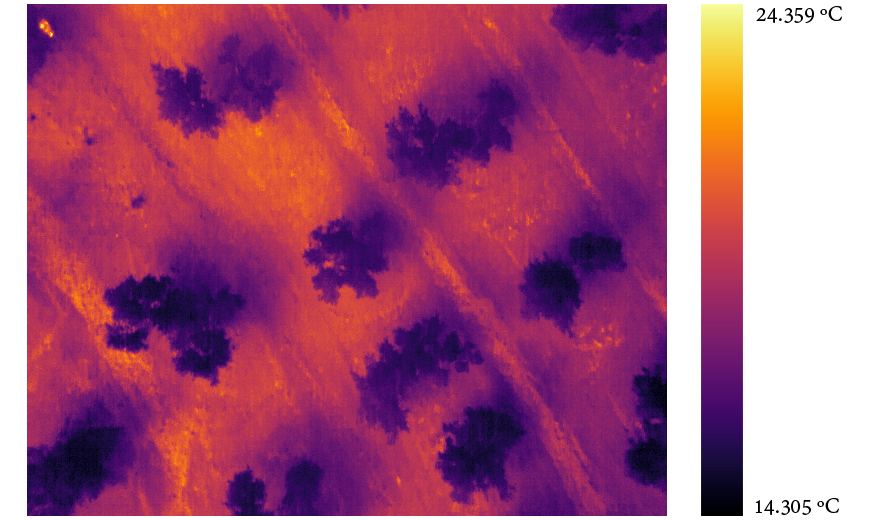
\includegraphics[width=\linewidth]{figs/materials/thermal_inferno_temperature.png}
	\caption{Normalized thermographic image encoded with the inferno colour-ramp texture. }
	\label{fig:thermal_inferno_temperature}
\end{figure}

\subsection{Nano-Hyperspec}

Nano-Hyperspec is a push-broom sensor that acquires spectral information for each spatial line. Light enters through the lens and it is dispersed in the spectral axis, thus allowing the observation of the spectra with a dimensionality of 640 spatial pixels. From here, the area is scanned following a flight direction and generating up to 2000 spatial lines per swath. If scanning the area requires more than 2000 spatial lines, several swaths are obtained for each sweep. 272 bands are acquired for every pixel covering a spectral interval ranging from 400 to 1,000 \si{\nano\meter}. The sampling frequency is 2.2 \si{\nano\meter}, though it increases to 6 \si{\nano\meter} at half-maximum.

\begin{marginfigure}[-3.0cm]
	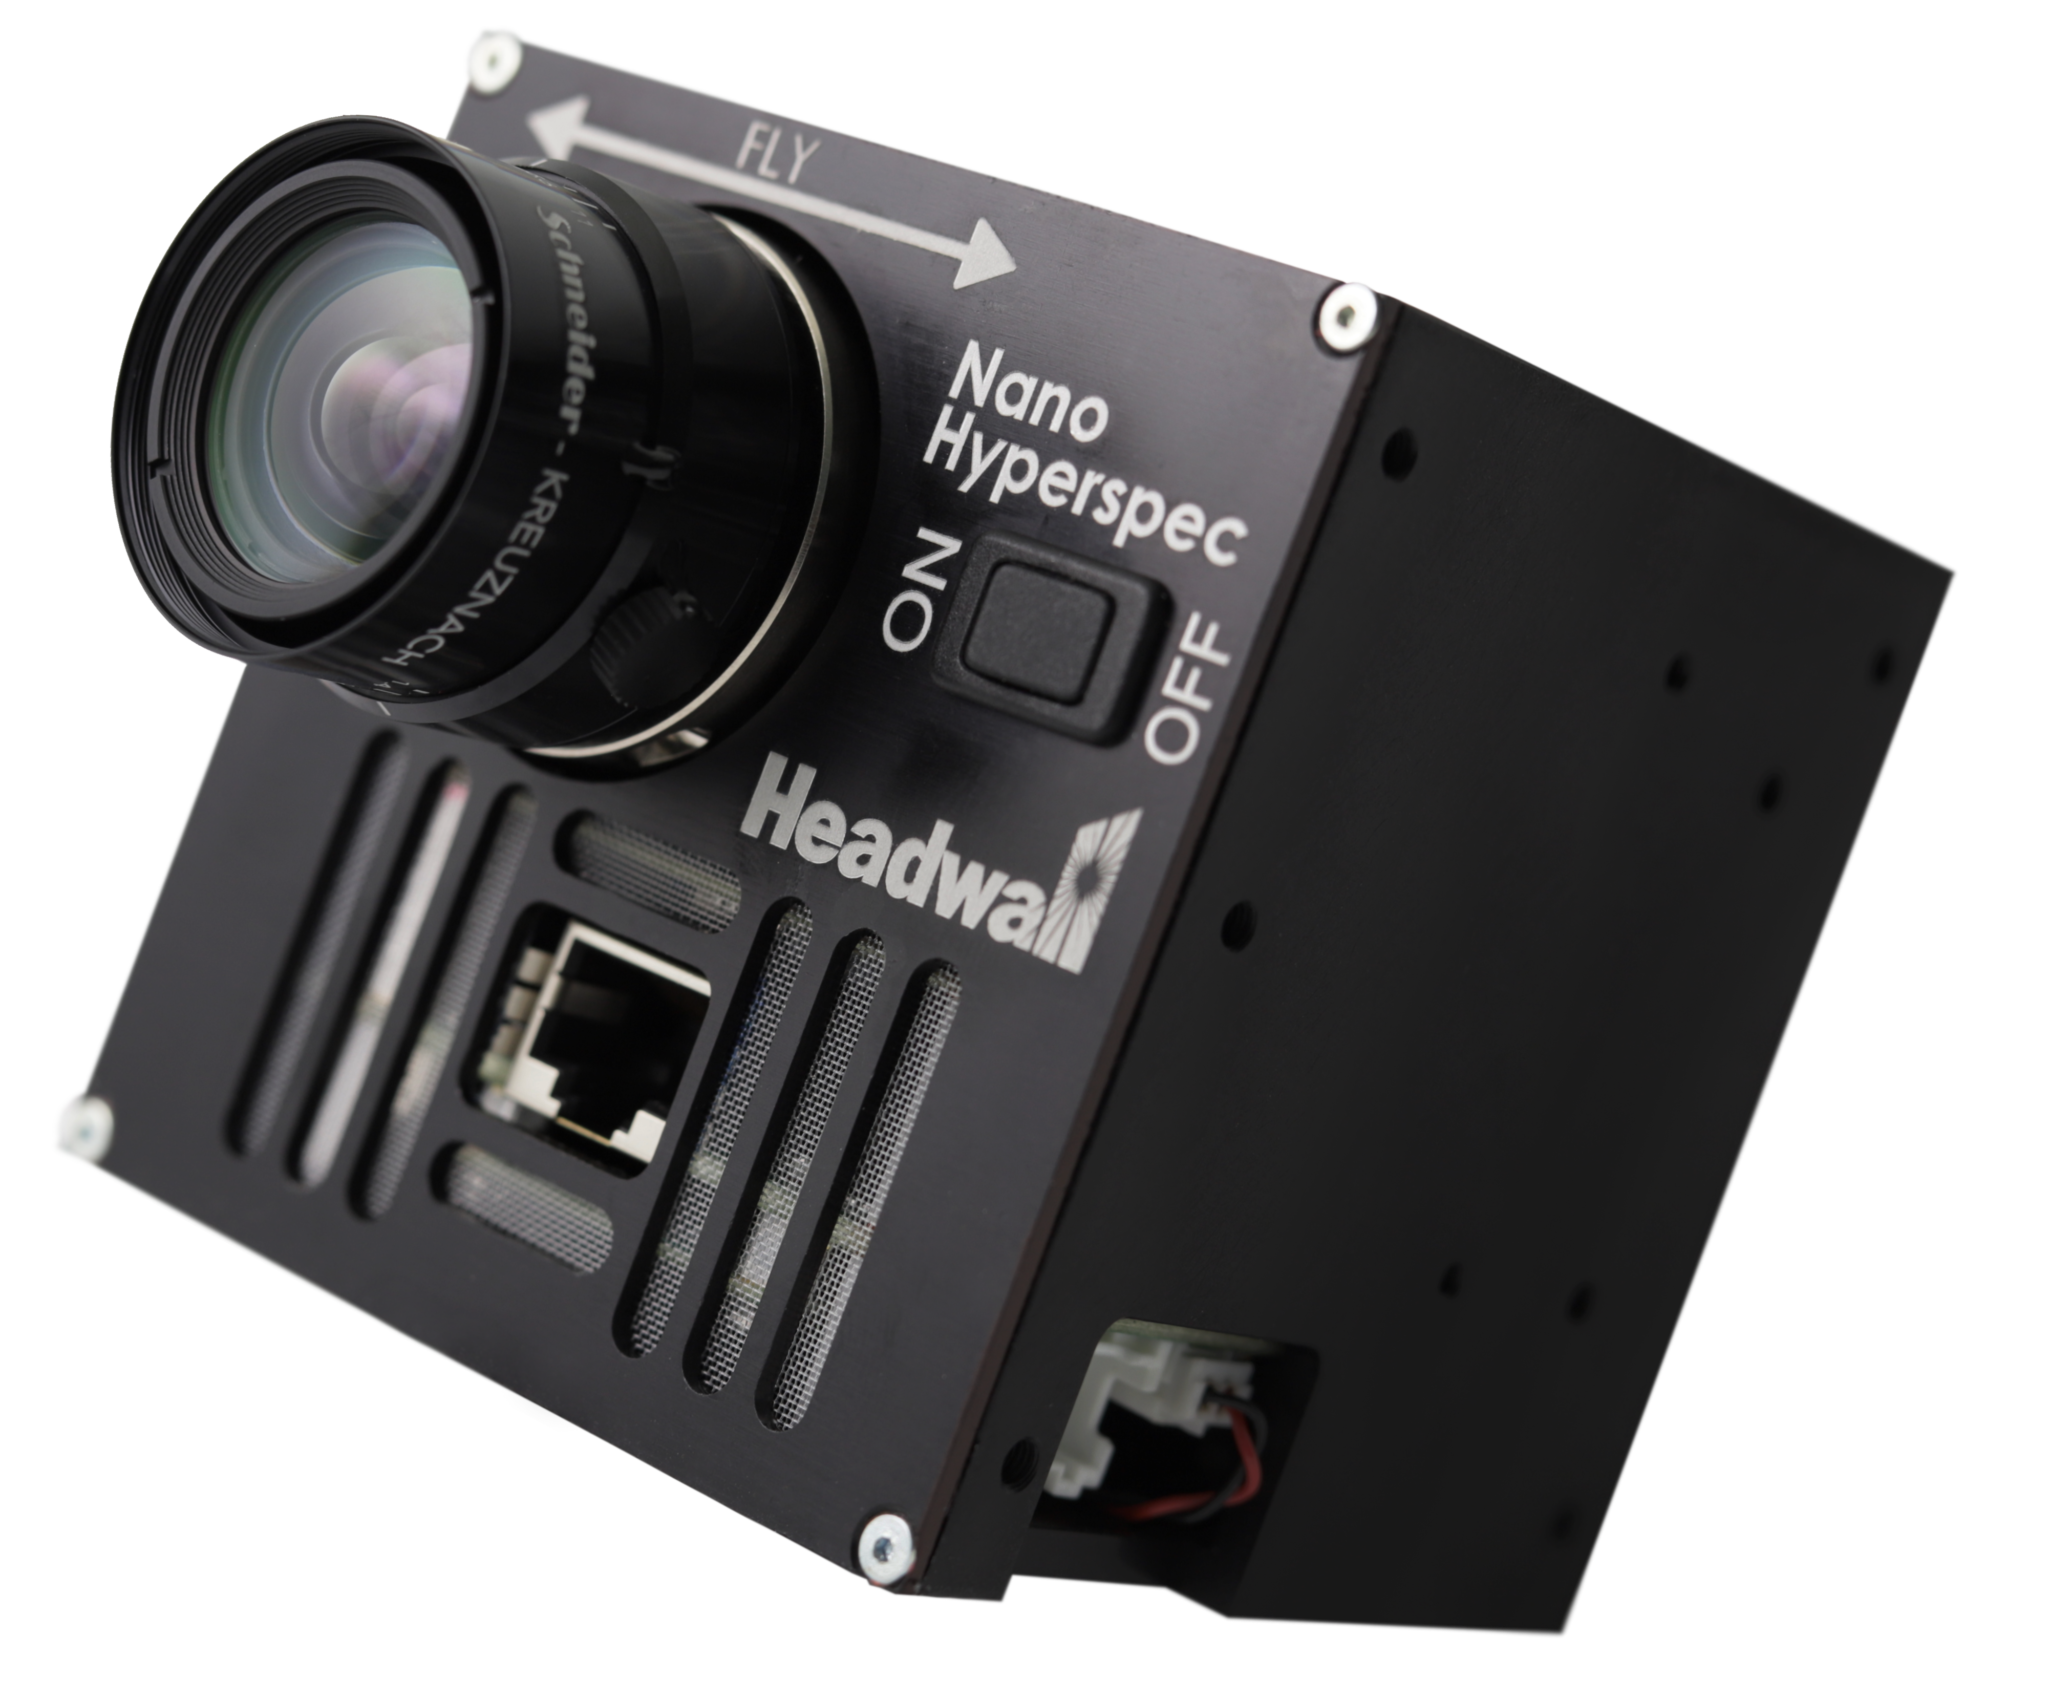
\includegraphics{figs/materials/nano_hyperspec.png}
	\caption{Nano-Hyperspec sensor.}
	\label{fig:nano_hyperspec}
\end{marginfigure}

The processing of hyperspectral data has been performed with Headwall SpectralView\texttrademark \hspace{1mm} software. The data collection procedure returns several swaths for each study area, with a grayscale tarp visible in at least one of them. Then, a white sample is marked from the white area in the grayscale tarp, while the dark reference is obtained by collecting a hyperspectral sample with the lens cap on before the flight. The sensor exposure and frame period are also adjusted before the flight by pointing at a bright reference to avoid clamping samples from white surfaces. The white and dark references are then used to convert the raw data to reflectance. 

\begin{figure*}[ht]
    \centering
    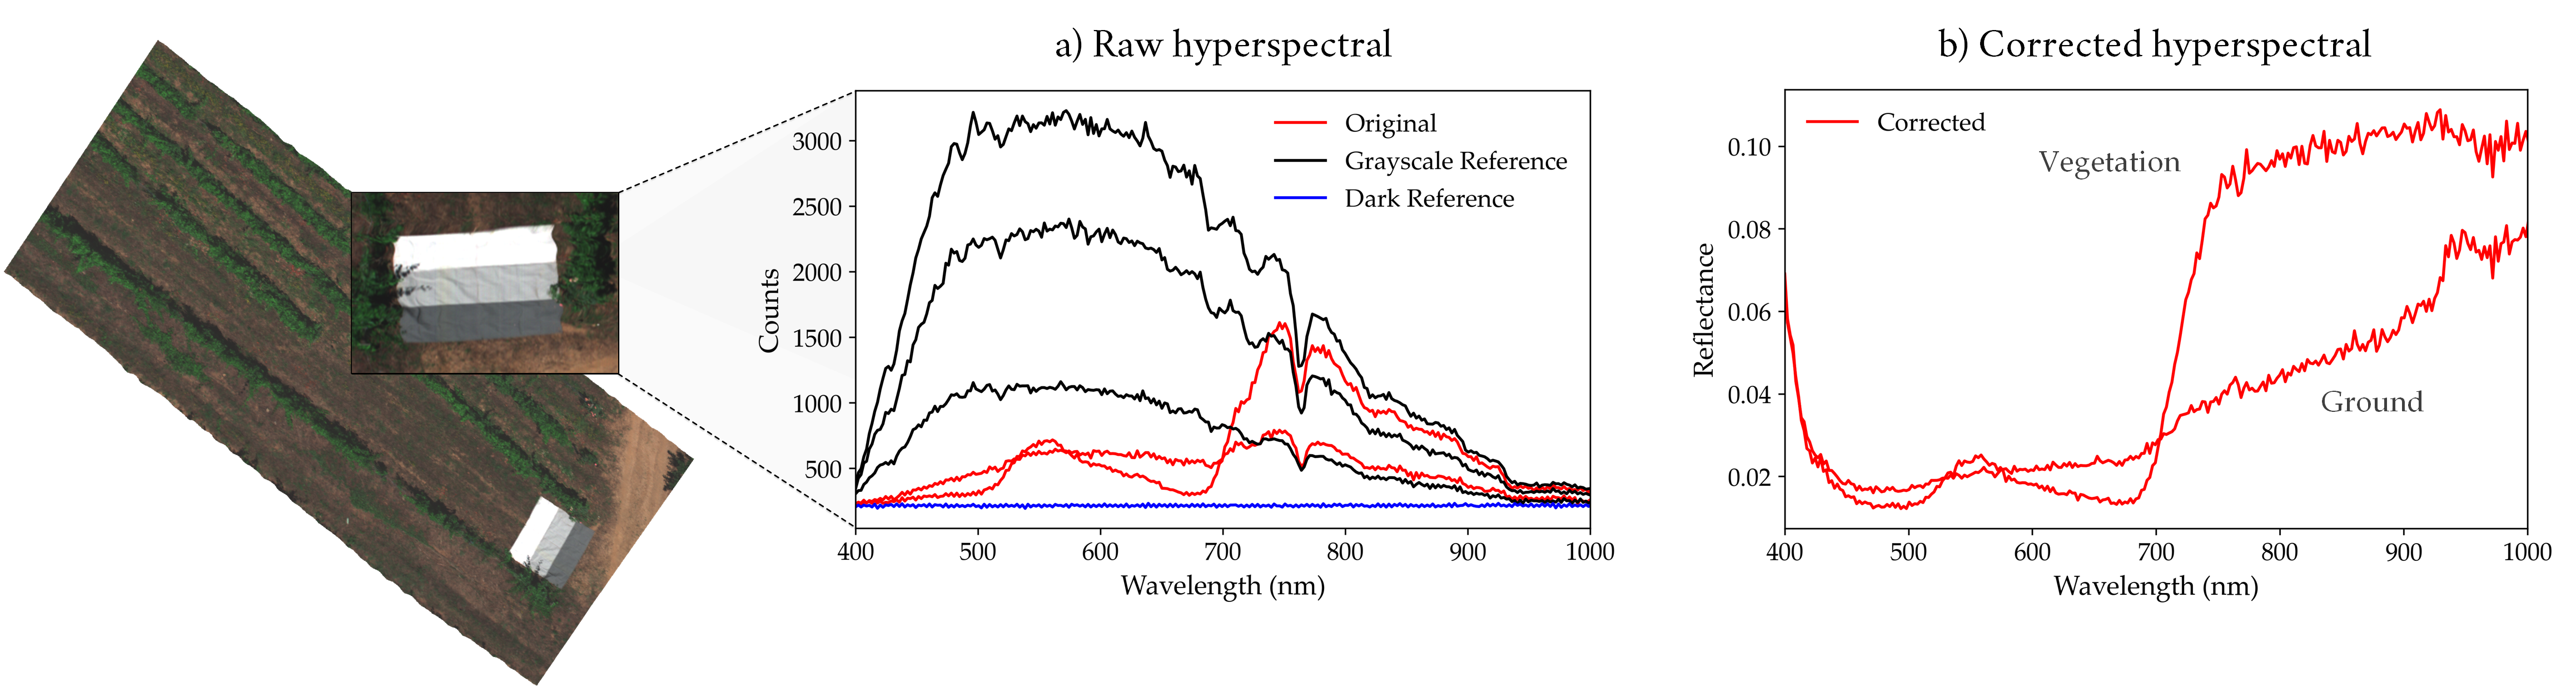
\includegraphics{figs/materials/spectral_view_rectification.png}
    \caption{Conversion of a) hyperspectral \acrshort{dn}s into b) reflectance using a white and dark reference. The three grey levels are sampled from a).}
    \label{fig:hyperspectral_rectification}
\end{figure*}

Ortho-rectified swaths are calculated using high-resolution \acrshort{dem}s (25 \si{\meter}) from Copernicus' observation program \cite{european_environment_agency_eu_2017} and the drone's \acrshort{gps} and \acrshort{imu} data. However, non-ortho-rectified swaths have also been used in this work for analysis to avoid distorting the hyperspectral samples and working with smaller image sizes.

\FloatBarrier
\begin{figure}[H]
    \centering
    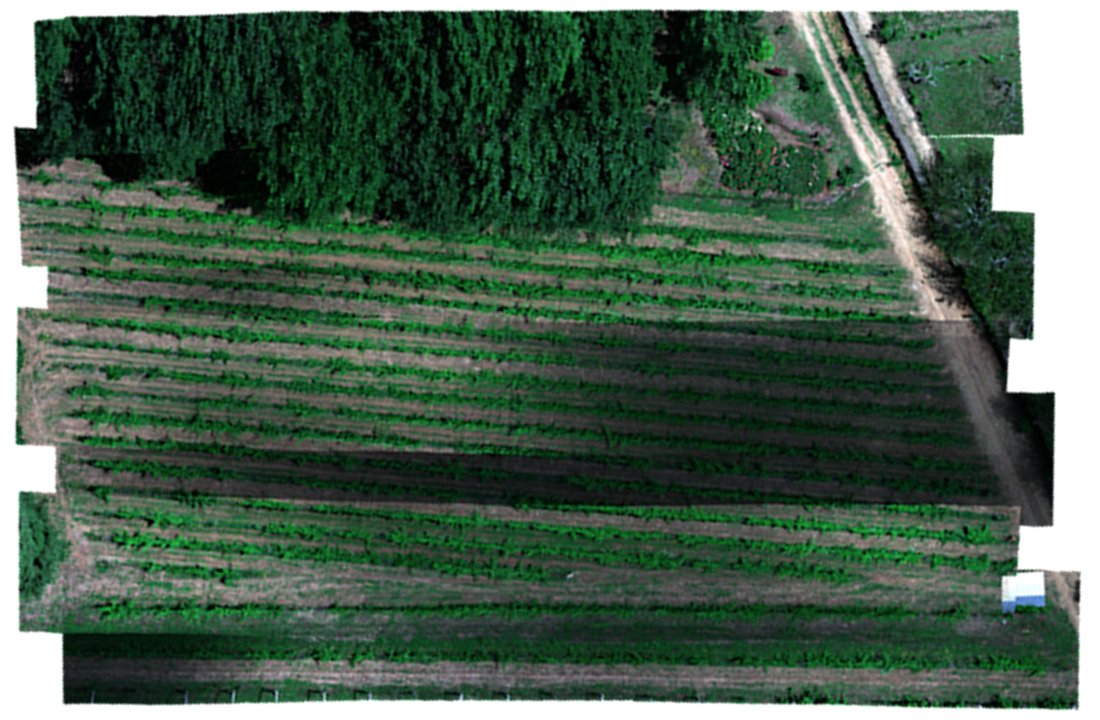
\includegraphics[width=0.8\linewidth]{figs/materials/orthorectified_hyper.png}
    \caption{Hyperspectral orthomosaic obtained by adjusting the yaw, roll and pitch angles as well as the \acrshort{uas}'s altitude in SpectralView\texttrademark \hspace{.3mm} software for every swath.}
    \label{fig:orthorectified_hyper}
\end{figure}

